\documentclass[tikz,border=10pt]{standalone}
\usetikzlibrary{calc}

\begin{document}

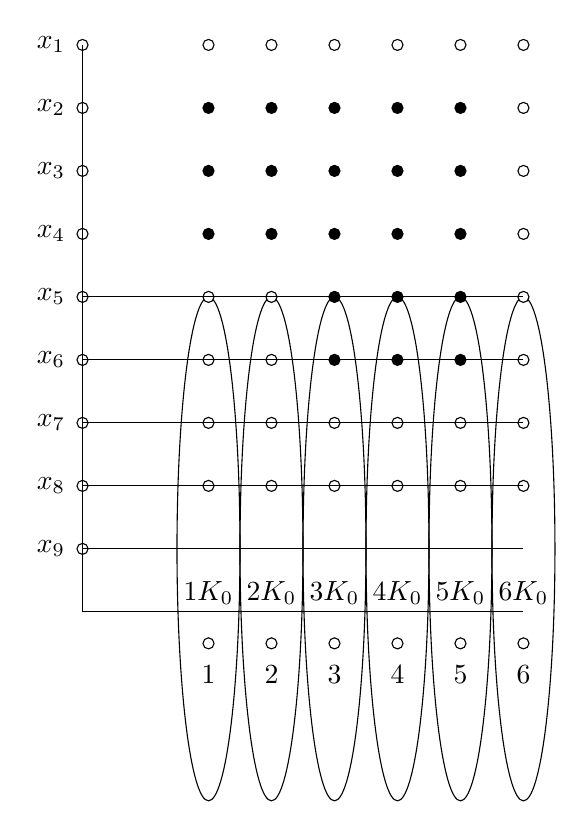
\begin{tikzpicture}[scale=0.8]
  % Styles
  \tikzset{
    vertex/.style={circle, draw, minimum size=4pt, inner sep=0pt},
    filled/.style={vertex, fill=black},
    empty/.style={vertex, fill=white}
  }
  
  % Left axis and labels
  \draw (0,0) -- (0,9);
  \foreach \i in {1,...,9} {
    \node at (-0.5,10-\i) {$x_{\i}$};
    \node[vertex] at (0,10-\i) {};
  }
  
  % Bottom axis and labels
  \draw (0,0) -- (7,0);
  \foreach \i in {1,...,6} {
    \node at (\i+1,-1) {$\i$};
    \node[vertex] at (\i+1,-0.5) {};
  }
  
  % Ellipses
  \foreach \i in {1,...,6} {
    \draw (\i+1,1) ellipse (0.5 and 4);
    \node at (\i+1,0.3) {$\i K_0$};
  }
  
  % Nodes and connections
  % 1K0 column
  \node[empty] at (2,9) {};
  \node[filled] at (2,8) {};
  \node[filled] at (2,7) {};
  \node[filled] at (2,6) {};
  \node[empty] at (2,5) {};
  \node[empty] at (2,4) {};
  \node[empty] at (2,3) {};
  \node[empty] at (2,2) {};
  
  % 2K0 column
  \node[empty] at (3,9) {};
  \node[filled] at (3,8) {};
  \node[filled] at (3,7) {};
  \node[filled] at (3,6) {};
  \node[empty] at (3,5) {};
  \node[empty] at (3,4) {};
  \node[empty] at (3,3) {};
  \node[empty] at (3,2) {};
  
  % 3K0 column
  \node[empty] at (4,9) {};
  \node[filled] at (4,8) {};
  \node[filled] at (4,7) {};
  \node[filled] at (4,6) {};
  \node[filled] at (4,5) {};
  \node[filled] at (4,4) {};
  \node[empty] at (4,3) {};
  \node[empty] at (4,2) {};
  
  % 4K0 column
  \node[empty] at (5,9) {};
  \node[filled] at (5,8) {};
  \node[filled] at (5,7) {};
  \node[filled] at (5,6) {};
  \node[filled] at (5,5) {};
  \node[filled] at (5,4) {};
  \node[empty] at (5,3) {};
  \node[empty] at (5,2) {};
  
  % 5K0 column
  \node[empty] at (6,9) {};
  \node[filled] at (6,8) {};
  \node[filled] at (6,7) {};
  \node[filled] at (6,6) {};
  \node[filled] at (6,5) {};
  \node[filled] at (6,4) {};
  \node[empty] at (6,3) {};
  \node[empty] at (6,2) {};
  
  % 6K0 column
  \node[empty] at (7,9) {};
  \node[empty] at (7,8) {};
  \node[empty] at (7,7) {};
  \node[empty] at (7,6) {};
  \node[empty] at (7,5) {};
  \node[empty] at (7,4) {};
  \node[empty] at (7,3) {};
  \node[empty] at (7,2) {};
  
  % Connections
  \foreach \i in {5,...,9} {
    \draw (0,10-\i) -- (2,10-\i);
    \draw (0,10-\i) -- (3,10-\i);
    \draw (0,10-\i) -- (4,10-\i);
    \draw (0,10-\i) -- (5,10-\i);
    \draw (0,10-\i) -- (6,10-\i);
    \draw (0,10-\i) -- (7,10-\i);
  }
  
\end{tikzpicture}

\end{document}